% FILE: Integrated multi-system models — coupled system dynamics, whole-organism simulation
\chapter{Integrated Multi-System Models}
\label{ch:integrated-systems}

The preceding chapters developed models of individual physiological subsystems in isolation. ME/CFS, however, is fundamentally a multi-system disease: energy metabolism, immune function, neuroendocrine regulation, and autonomic control are coupled through shared substrates, signaling molecules, and feedback loops (Chapter~\ref{ch:integrative-models}). This chapter formalizes the inter-system couplings and constructs an integrated model that captures emergent properties not present in any subsystem alone.

% Figure: Whole-Body ME/CFS Systems Model Architecture
% Shows 7 subsystem modules in circular layout with labeled coupling arrows

\begin{figure}[htbp]
\centering
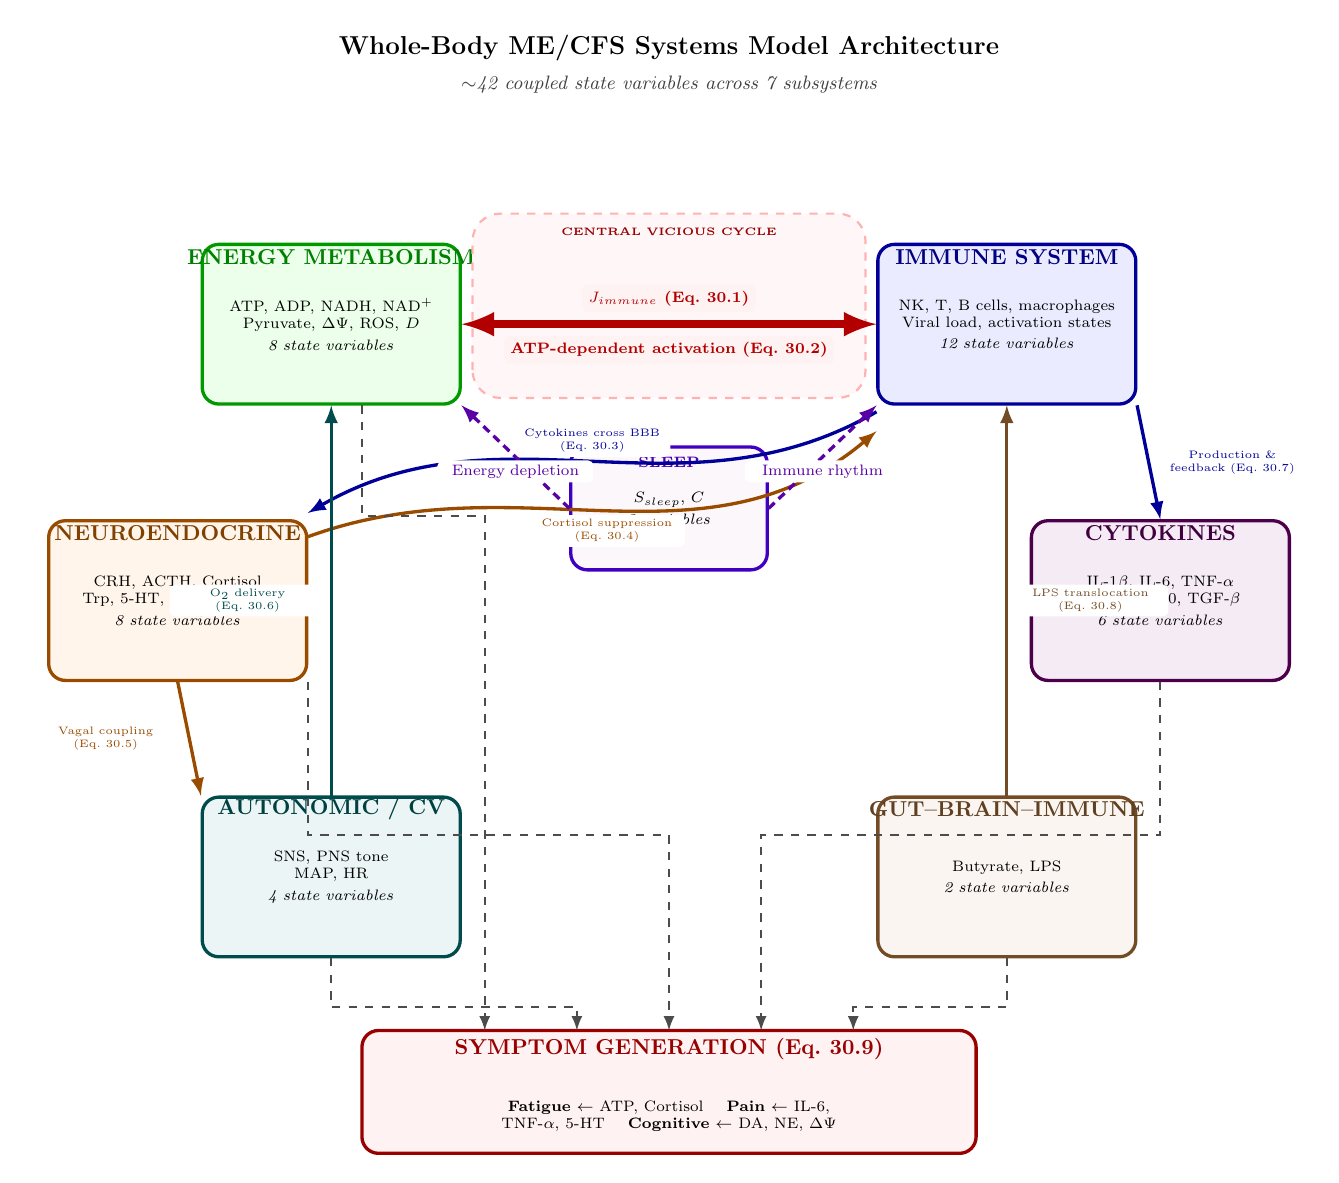
\begin{tikzpicture}[
    scale=0.78, every node/.style={scale=0.78},
    % Subsystem box styles
    subsystem/.style={draw=black!70, very thick, rounded corners=6pt,
        minimum width=4.2cm, minimum height=2.6cm, align=center, inner sep=5pt},
    energy-sys/.style={subsystem, draw=green!60!black, fill=green!8},
    immune-sys/.style={subsystem, draw=blue!60!black, fill=blue!8},
    cytokine-sys/.style={subsystem, draw=violet!60!black, fill=violet!8},
    neuro-sys/.style={subsystem, draw=orange!60!black, fill=orange!8},
    auto-sys/.style={subsystem, draw=teal!60!black, fill=teal!8},
    gut-sys/.style={subsystem, draw=brown!60!black, fill=brown!8},
    sleep-sys/.style={subsystem, draw=blue!50!violet, fill=blue!3!violet!3,
        minimum width=3.2cm, minimum height=2cm},
    symptom-sys/.style={draw=red!60!black, fill=red!5, very thick,
        rounded corners=6pt, minimum width=10cm, minimum height=2cm,
        align=center, inner sep=5pt},
    % Arrow styles
    coupling/.style={-latex, thick, line width=1.2pt},
    vicious/.style={latex-latex, ultra thick, red!70!black, line width=3pt},
    symptom-arrow/.style={-latex, thick, dashed, gray!60!black},
    % Label styles
    mechanism/.style={font=\tiny, fill=white, inner sep=2pt, rounded corners=2pt,
        text width=2.4cm, align=center},
]

% === TITLE ===
\node[font=\large\bfseries] at (0, 10.5) {Whole-Body ME/CFS Systems Model Architecture};
\node[font=\small\itshape, gray!50!black] at (0, 9.9) {$\sim$42 coupled state variables across 7 subsystems};

% === SUBSYSTEM NODES (circular layout) ===
% Energy Metabolism (top-left)
\node[energy-sys] (energy) at (-5.5, 6) {};
\node[font=\bfseries, green!50!black] at (-5.5, 7.1) {ENERGY METABOLISM};
\node[font=\scriptsize, text width=3.8cm, align=center] at (-5.5, 6) {
    ATP, ADP, NADH, NAD\textsuperscript{+}\\
    Pyruvate, $\Delta\Psi$, ROS, $D$\\[2pt]
    \textit{8 state variables}
};

% Immune System (top-right)
\node[immune-sys] (immune) at (5.5, 6) {};
\node[font=\bfseries, blue!50!black] at (5.5, 7.1) {IMMUNE SYSTEM};
\node[font=\scriptsize, text width=3.8cm, align=center] at (5.5, 6) {
    NK, T, B cells, macrophages\\
    Viral load, activation states\\[2pt]
    \textit{12 state variables}
};

% Cytokines (right)
\node[cytokine-sys] (cytokine) at (8, 1.5) {};
\node[font=\bfseries, violet!50!black] at (8, 2.6) {CYTOKINES};
\node[font=\scriptsize, text width=3.8cm, align=center] at (8, 1.5) {
    IL-1$\beta$, IL-6, TNF-$\alpha$\\
    IFN-$\gamma$, IL-10, TGF-$\beta$\\[2pt]
    \textit{6 state variables}
};

% Neuroendocrine (left)
\node[neuro-sys] (neuro) at (-8, 1.5) {};
\node[font=\bfseries, orange!50!black] at (-8, 2.6) {NEUROENDOCRINE};
\node[font=\scriptsize, text width=3.8cm, align=center] at (-8, 1.5) {
    CRH, ACTH, Cortisol\\
    Trp, 5-HT, Kyn, DA, NE\\[2pt]
    \textit{8 state variables}
};

% Autonomic/Cardiovascular (bottom-left)
\node[auto-sys] (auto) at (-5.5, -3) {};
\node[font=\bfseries, teal!50!black] at (-5.5, -1.9) {AUTONOMIC / CV};
\node[font=\scriptsize, text width=3.8cm, align=center] at (-5.5, -3) {
    SNS, PNS tone\\
    MAP, HR\\[2pt]
    \textit{4 state variables}
};

% Gut-Brain-Immune (bottom-right)
\node[gut-sys] (gut) at (5.5, -3) {};
\node[font=\bfseries, brown!50!black] at (5.5, -1.9) {GUT--BRAIN--IMMUNE};
\node[font=\scriptsize, text width=3.8cm, align=center] at (5.5, -3) {
    Butyrate, LPS\\[2pt]
    \textit{2 state variables}
};

% Sleep (small, upper center)
\node[sleep-sys] (sleep) at (0, 3) {};
\node[font=\bfseries\scriptsize, blue!40!violet] at (0, 3.75) {SLEEP};
\node[font=\scriptsize, text width=2.8cm, align=center] at (0, 3) {
    $S_{\text{sleep}}$, $C$\\[2pt]
    \textit{2 variables}
};

% === CENTRAL VICIOUS CYCLE (Energy <-> Immune) ===
% Highlight box
\draw[red!30, fill=red!3, rounded corners=10pt, dashed, thick]
    (-3.2, 4.8) rectangle (3.2, 7.8);
\node[font=\tiny\bfseries, red!60!black] at (0, 7.5) {CENTRAL VICIOUS CYCLE};

% Bidirectional red arrows
\draw[vicious] (energy.east) -- (immune.west)
    node[midway, above=4pt, font=\scriptsize\bfseries, red!70!black, fill=red!5,
        rounded corners=2pt, inner sep=3pt] {$J_{\text{immune}}$ (Eq.~30.1)}
    node[midway, below=4pt, font=\scriptsize\bfseries, red!70!black, fill=red!5,
        rounded corners=2pt, inner sep=3pt] {ATP-dependent activation (Eq.~30.2)};

% === COUPLING ARROWS ===

% Immune -> Neuroendocrine (cytokines cross BBB)
% Route: from immune south-west corner, curving down to neuro north-east corner
\draw[coupling, blue!60!black]
    ([yshift=-3pt]immune.south west) to[out=210, in=30]
    node[mechanism, pos=0.5, above=2pt] {Cytokines cross BBB\\(Eq.~30.3)}
    ([yshift=3pt]neuro.north east);

% Neuroendocrine -> Immune (cortisol suppression)
% Route: from neuro north-east, curving up to immune south-west — offset to avoid overlap
\draw[coupling, orange!60!black]
    ([yshift=-8pt]neuro.north east) to[out=20, in=220]
    node[mechanism, pos=0.5, below=2pt] {Cortisol suppression\\(Eq.~30.4)}
    ([yshift=-12pt]immune.south west);

% Neuroendocrine -> Autonomic (vagal coupling)
\draw[coupling, orange!60!black] (neuro.south) -- (auto.north west)
    node[mechanism, pos=0.5, left=2pt] {Vagal coupling\\(Eq.~30.5)};

% Autonomic -> Energy (O2 delivery)
\draw[coupling, teal!60!black] (auto.north) -- (energy.south)
    node[mechanism, pos=0.5, left=2pt] {O\textsubscript{2} delivery\\(Eq.~30.6)};

% Immune <-> Cytokines (production and feedback)
\draw[coupling, blue!60!black] (immune.south east) -- (cytokine.north)
    node[mechanism, pos=0.5, right=2pt] {Production \&\\feedback (Eq.~30.7)};

% Gut -> Immune (LPS translocation)
\draw[coupling, brown!60!black] (gut.north) -- (immune.south)
    node[mechanism, pos=0.5, right=2pt] {LPS translocation\\(Eq.~30.8)};

% Sleep connections (lighter)
\draw[coupling, blue!30!violet, densely dashed] (sleep.west) -- (energy.south east)
    node[mechanism, pos=0.5, below=1pt] {\scriptsize Energy depletion};
\draw[coupling, blue!30!violet, densely dashed] (sleep.east) -- (immune.south west)
    node[mechanism, pos=0.5, below=1pt] {\scriptsize Immune rhythm};

% === SYMPTOM GENERATION MODULE (bottom) ===
\node[symptom-sys] (symptoms) at (0, -6.5) {};
\node[font=\bfseries, red!60!black] at (0, -5.8) {SYMPTOM GENERATION (Eq.~30.9)};
\node[font=\scriptsize, text width=9cm, align=center] at (0, -6.9) {
    \textbf{Fatigue} $\leftarrow$ ATP, Cortisol \quad
    \textbf{Pain} $\leftarrow$ IL-6, TNF-$\alpha$, 5-HT \quad
    \textbf{Cognitive} $\leftarrow$ DA, NE, $\Delta\Psi$
};

% Symptom input arrows
\draw[symptom-arrow] (energy.south) ++(0.5,0) -- ++(0,-1.8) -| (-3, -5.5);
\draw[symptom-arrow] (auto.south) -- ++(0,-0.8) -| (-1.5, -5.5);
\draw[symptom-arrow] (neuro.south east) -- ++(0,-2.5) -| (0, -5.5);
\draw[symptom-arrow] (cytokine.south) -- ++(0,-2.5) -| (1.5, -5.5);
\draw[symptom-arrow] (gut.south) -- ++(0,-0.8) -| (3, -5.5);

\end{tikzpicture}
\caption{Architecture of the integrated whole-body model showing subsystem modules
and their couplings. The central energy--immune vicious cycle (red) drives disease
persistence. Arrows indicate the dominant coupling direction; most interactions are
bidirectional. The symptom generation module (bottom) maps physiological states to
clinical symptoms.}
\label{fig:integrated-systems-architecture}
\end{figure}


\section{Energy--Immune Coupling}
\label{sec:energy-immune-coupling}

The bidirectional coupling between energy metabolism and immune function constitutes the most critical feedback loop in ME/CFS pathophysiology. The coupling operates through two channels.

\subsection{Immune Activation Drains Energy}

Activated immune cells consume substantial ATP, as quantified by the immune energy demand term $J_{\text{immune}}$ (Equation~\ref{eq:immune-energy}). This demand enters the ATP balance (Equation~\ref{eq:atp-balance}) directly:

\begin{equation}
\label{eq:energy-immune-coupling}
\frac{d[\text{ATP}]}{dt} = J_{\text{production}} - J_{\text{basal}} - J_{\text{activity}}(t) - J_{\text{immune}}(N_a, M_a, T_a)
\end{equation}

where $J_{\text{immune}}$ depends on the activated cell populations from the immune model (Chapter~\ref{ch:immune-system-models}). During immune flares, $J_{\text{immune}}$ can increase several-fold, consuming energy that would otherwise be available for physical and cognitive activity. This provides a mechanistic explanation for the observation that ME/CFS symptoms worsen during infections or immune activation episodes.

\subsection{Energy Deficits Impair Immunity}

The reverse coupling is equally important: immune cell function depends on adequate energy supply. NK cell cytotoxicity, T~cell proliferation, and antibody production all require ATP. When $[\text{ATP}]$ falls below a functional threshold, immune cell performance degrades:

\begin{equation}
\label{eq:immune-energy-feedback}
k_{\text{act}}^{\text{eff}} = k_{\text{act}} \cdot \frac{[\text{ATP}]^2}{K_{\text{ATP,immune}}^2 + [\text{ATP}]^2}
\end{equation}

where $k_{\text{act}}^{\text{eff}}$ is the effective immune activation rate and the Hill function (exponent~2) represents the cooperative dependence on ATP availability. This creates the central vicious cycle of ME/CFS: immune activation $\to$ energy depletion $\to$ impaired immune control $\to$ persistent infection/autoimmunity $\to$ sustained immune activation. The coupled model predicts that this cycle is self-sustaining above a critical level of immune activation---below this threshold, the healthy state is stable; above it, the system converges to a pathological attractor.

\begin{hypothesis}[Bistability of the Energy--Immune Cycle]
The coupled energy--immune system exhibits bistability: a healthy attractor (low immune activation, adequate energy) and a disease attractor (chronic immune activation, energy deficit) coexist for the same parameter values. The transition from health to disease occurs when a sufficiently strong perturbation (e.g., acute infection) pushes the system past a separatrix into the basin of attraction of the disease state. Recovery requires a perturbation of comparable magnitude in the reverse direction---or a sustained intervention that eliminates the disease attractor entirely by modifying system parameters (e.g., sufficient immunosuppression to break the cycle). This model predicts that: (1)~disease onset is triggered by events exceeding a threshold severity, not by any specific pathogen; (2)~spontaneous recovery is rare because the disease attractor is stable; and (3)~effective treatment must be sustained long enough to shift the system past the separatrix, explaining why brief interventions often fail.

\textbf{Certainty}: 0.50. Bistability is a natural consequence of the positive feedback structure and is consistent with the clinical observation that ME/CFS often begins with an acute trigger but persists indefinitely. Direct demonstration of bistability would require longitudinal measurement of both immune and metabolic variables with sufficient temporal resolution to map the state-space trajectory.
\end{hypothesis}

\section{Neuroimmune Interactions}
\label{sec:neuroimmune-interactions}

The neuroimmune coupling operates through three pathways, each with distinct timescales.

\subsection{Cytokine Effects on Brain Function}

Peripheral cytokines affect CNS function through two mechanisms modeled in Chapter~\ref{ch:immune-system-models}: (1)~transport across the blood--brain barrier (Equation~\ref{eq:bbb-transport}), and (2)~activation of vagal afferents that signal to the brainstem~\cite{Dantzer2007twenty}. Once in the CNS, pro-inflammatory cytokines activate microglia (Equation~\ref{eq:microglia}), disrupt neurotransmitter synthesis (Equations~\ref{eq:tryptophan}--\ref{eq:ido-regulation}), and alter HPA axis function (through direct effects on hypothalamic CRH neurons). The integrated model connects these pathways:

\begin{equation}
\label{eq:neuroimmune-cns}
\boldsymbol{C}_{\text{CNS}}(t) = P_{\text{BBB}}(t) \cdot \boldsymbol{C}_{\text{plasma}}(t) + \boldsymbol{T}_{\text{active}} + \boldsymbol{C}_{\text{local}}(\mu_1)
\end{equation}

where $\boldsymbol{C}_{\text{local}}(\mu_1)$ represents cytokines produced locally by activated microglia. Equation~\ref{eq:neuroimmune-cns} is a quasi-steady-state approximation of the full transport dynamics (Equation~\ref{eq:bbb-transport}), valid when CNS cytokine turnover is fast relative to BBB permeability changes. The CNS cytokine environment then modulates neurotransmitter dynamics, autonomic output, and HPA axis function---creating a pathway from peripheral immune activation to cognitive dysfunction, sleep disturbance, and autonomic symptoms.

\subsection{HPA Axis and Immune Regulation}

Cortisol from the HPA axis model (Equation~\ref{eq:hpa-axis}) feeds back to the immune system as a major anti-inflammatory signal:

\begin{equation}
\label{eq:cortisol-immune}
\sigma_{\text{cytokine},i}^{\text{eff}} = \sigma_{\text{cytokine},i} \cdot \frac{K_F^{\text{immune}}}{K_F^{\text{immune}} + F}
\end{equation}

where the cortisol concentration $F$ inhibits pro-inflammatory cytokine production. The reduced cortisol output in ME/CFS (Section~\ref{sec:hpa-dysfunction-model}) weakens this inhibitory brake, permitting higher cytokine levels than would otherwise be sustained. This neuroimmune coupling explains why stress management---by reducing cortisol demand---and low-dose hydrocortisone replacement have shown limited benefit in some ME/CFS patients.

\subsection{Vagal Signaling}

The vagus nerve provides a rapid bidirectional communication pathway between the periphery and the CNS. Afferent vagal fibers detect peripheral cytokines (particularly IL-1$\beta$ and TNF-$\alpha$) and transmit inflammatory signals to the nucleus tractus solitarius (NTS)~\cite{Marty2008NTS}, producing sickness behavior (fatigue, anorexia, social withdrawal). Efferent vagal fibers mediate the cholinergic anti-inflammatory pathway, suppressing macrophage TNF-$\alpha$ production through $\alpha$7 nicotinic acetylcholine receptors~\cite{Huerta2025vagal}. The vagal coupling is modeled as:

\begin{equation}
\label{eq:vagal-coupling}
\sigma_{\text{TNF}}^{\text{eff}} = \sigma_{\text{TNF}} \cdot \frac{K_{\text{vagal}}}{K_{\text{vagal}} + V_{\text{efferent}}}
\end{equation}

where $V_{\text{efferent}}$ is vagal efferent tone from the ANS model (Equation~\ref{eq:ans-balance}). Reduced vagal tone in ME/CFS therefore diminishes the cholinergic anti-inflammatory pathway, providing an additional mechanism for sustained peripheral inflammation.

\section{Cardiovascular--Metabolic Integration}
\label{sec:cardiovascular-metabolic}

Oxygen delivery to tissues depends on cardiac output, blood oxygen content, and microvascular perfusion. The cardiovascular--metabolic coupling links the autonomic model (heart rate, blood pressure) to the energy metabolism model (oxygen-dependent ATP production):

\begin{equation}
\label{eq:o2-delivery}
\text{DO}_2 = \text{CO} \cdot \text{CaO}_2 = (\text{HR} \cdot \text{SV}) \cdot (1.34 \cdot [\text{Hb}] \cdot \text{SaO}_2 + 0.003 \cdot \text{PaO}_2)
\end{equation}

where DO$_2$ is oxygen delivery, CO is cardiac output (heart rate $\times$ stroke volume), and CaO$_2$ is arterial oxygen content. Tissue oxygen extraction determines the available oxygen for mitochondrial respiration:

\begin{equation}
\label{eq:o2-consumption}
\text{VO}_2 = \text{DO}_2 \cdot \text{O}_2\text{ER} = \text{DO}_2 \cdot \frac{\text{CaO}_2 - \text{CvO}_2}{\text{CaO}_2}
\end{equation}

In ME/CFS, reduced cardiac output (due to autonomic dysfunction and hypovolemia), impaired oxygen extraction (due to microvascular dysfunction or mitochondrial uncoupling), or both can reduce tissue VO$_2$. The oxygen consumption $\text{VO}_2$ constrains the maximal ETC flux in the energy model: $J_{\text{CIV,max}} \propto \text{VO}_2$. Reduced cerebral blood flow has been documented in ME/CFS patients~\cite{Novak2022CBFReview}, suggesting that the brain may be particularly vulnerable to this cardiovascular--metabolic mismatch.

\section{Gut--Brain--Immune Axis}
\label{sec:gut-brain-immune-axis}

Gut microbiome alterations in ME/CFS (Chapter~\ref{ch:gut-microbiome}) affect both immune function and CNS signaling through multiple pathways. The integrated model includes three gut-derived signals:

\begin{enumerate}
    \item \textbf{Short-chain fatty acids (SCFAs)}: Butyrate, produced by commensal bacteria, maintains intestinal barrier integrity and exerts anti-inflammatory effects~\cite{Folkerts2020butyrate}. Reduced butyrate-producing bacteria in ME/CFS~\cite{Hsu2025gut} is modeled as decreased $[\text{butyrate}]$, which increases intestinal permeability and permits translocation of bacterial products (lipopolysaccharide, LPS) into the circulation.
    \item \textbf{LPS-driven immune activation}: Translocated LPS activates monocytes/macrophages through TLR4, increasing pro-inflammatory cytokine production. This is an additional input to the cytokine network model (Equation~\ref{eq:cytokine-general}).
    \item \textbf{Microbiome-derived neurotransmitter precursors}: Gut bacteria produce tryptophan metabolites, GABA, and other neuroactive compounds that reach the CNS via the vagus nerve or systemic circulation, modulating the neurotransmitter models in Chapter~\ref{ch:neuroendocrine-models}.
\end{enumerate}

The gut--brain--immune axis coupling is modeled as:

\begin{equation}
\label{eq:gut-immune}
J_{\text{LPS}} = k_{\text{perm}} \cdot \frac{K_{\text{butyrate}}}{K_{\text{butyrate}} + [\text{butyrate}]} \cdot [\text{LPS}_{\text{gut}}]
\end{equation}

where intestinal permeability increases as butyrate decreases, allowing more LPS translocation. The circulating LPS then drives immune activation, which via the neuroimmune pathway affects CNS function. This chain provides a mechanistic link between gut dysbiosis and neurological symptoms in ME/CFS.

\subsection{GI Motility and SIBO Dynamics}
\label{sec:gi-motility-model}

GI dysmotility is a core component of the Septad framework (Section~\ref{sec:septad}). Gastric emptying scintigraphy studies report delayed emptying in approximately 60\% of tested ME/CFS patients~\cite{GastricDysmotility2023}, while breath testing identifies SIBO in 48\% of those evaluated~\cite{SIBOKarhu2023}. Gastroparesis and impaired migrating motor complex (MMC) function predispose to small intestinal bacterial overgrowth (SIBO), which in turn drives immune activation and nutrient malabsorption (Chapter~\ref{ch:gut-microbiome}, Section~\ref{sec:sibo}). The preceding gut--brain--immune model captures dysbiosis$\to$permeability$\to$LPS translocation but omits motility entirely. This subsection extends the gut compartment to formalize the autonomic$\to$motility$\to$SIBO$\to$immune$+$energy cascade.

The model tracks three additional state variables: gut motility index $\mathcal{G} \in [0,1]$ (where 1 is normal MMC cycling and 0 is complete gastroparesis), small intestinal bacterial load $B_{\text{SI}}$ (colony-forming units, normalized to healthy baseline $B_{\text{SI},0}$), and nutrient absorption efficiency $\eta \in [0,1]$:

\begin{align}
\label{eq:gi-motility}
\frac{d\mathcal{G}}{dt} &= \frac{1}{\tau_{\mathcal{G}}} \left[ \mathcal{G}_{\text{set}}(V, \text{MC}_d) + \mathcal{G}_{\text{pro}} - \mathcal{G} \right] \\[6pt]
\label{eq:sibo-dynamics}
\frac{dB_{\text{SI}}}{dt} &= r_B \cdot B_{\text{SI}} \left(1 - \frac{B_{\text{SI}}}{K_B(\mathcal{G})}\right) - \delta_{\text{MMC}} \cdot \mathcal{G}^2 \cdot B_{\text{SI}} - \delta_{\text{Abx}} \cdot B_{\text{SI}} \\[6pt]
\label{eq:absorption-efficiency}
\frac{d\eta}{dt} &= \frac{1}{\tau_\eta} \left[ \eta_0 \cdot \frac{K_\eta}{K_\eta + B_{\text{SI}}/B_{\text{SI},0}} - \eta \right]
\end{align}

In Equation~\ref{eq:gi-motility}, $\mathcal{G}_{\text{pro}} \geq 0$ represents the prokinetic drug effect (e.g., prucalopride, low-dose erythromycin), which directly augments motility independently of vagal tone; $\mathcal{G}_{\text{pro}} = 0$ in the absence of prokinetic treatment. The motility set point $\mathcal{G}_{\text{set}}$ depends on vagal efferent tone $V$ (from the ANS model, Equation~\ref{eq:ans-balance}) and mast cell degranulation state $\text{MC}_d$ (from the mast cell model, Equation~\ref{eq:mast-cell-dynamics}):

\begin{equation}
\label{eq:motility-setpoint}
\mathcal{G}_{\text{set}}(V, \text{MC}_d) = \underbrace{\frac{V^{n_V}}{K_V^{n_V} + V^{n_V}}}_{\text{vagal drive}} \cdot \underbrace{\frac{K_{\text{MC,gut}}}{K_{\text{MC,gut}} + \text{MC}_d}}_{\text{mast cell inhibition}}
\end{equation}

Vagal tone drives motility through the enteric nervous system: reduced vagal output (as in ME/CFS autonomic dysfunction) lowers the motility set point, impairing MMC cycling. Simultaneously, degranulated mast cells in the gut mucosa release histamine and prostaglandins that can disrupt coordinated peristalsis (Chapter~\ref{ch:gut-microbiome}). The Hill coefficient $n_V$ determines the steepness of the vagal drive---a steep response means that modest vagal impairment has disproportionate effects on motility, consistent with the clinical observation that many ME/CFS patients develop gastroparesis despite only moderate autonomic dysfunction.

In the SIBO dynamics (Equation~\ref{eq:sibo-dynamics}), bacterial growth follows logistic kinetics with a carrying capacity $K_B(\mathcal{G})$ that increases as motility decreases:

\begin{equation}
\label{eq:sibo-carrying-capacity}
K_B(\mathcal{G}) = K_{B,\text{min}} + (K_{B,\text{max}} - K_{B,\text{min}}) \cdot (1 - \mathcal{G})
\end{equation}

The MMC clearance term $\delta_{\text{MMC}} \cdot \mathcal{G}^2$ is quadratic in motility, reflecting the fact that effective bacterial sweep requires coordinated phase~III contractions---partial motility provides disproportionately less clearance. The antibiotic term $\delta_{\text{Abx}}$ represents rifaximin or herbal antimicrobial treatment (Section~\ref{sec:sibo}).

\subsubsection{Cross-System Coupling}

The GI motility model couples to four other subsystems:

\begin{enumerate}
    \item \textbf{SIBO $\to$ Immune activation}: Bacterial overgrowth increases luminal LPS concentration. The existing LPS translocation equation (Equation~\ref{eq:gut-immune}) is extended with a SIBO-dependent source term:
    \begin{equation}
    \label{eq:lps-sibo}
    [\text{LPS}_{\text{gut}}] = [\text{LPS}_{\text{gut},0}] \cdot \frac{B_{\text{SI}}}{B_{\text{SI},0}}
    \end{equation}
    This creates a positive feedback loop: autonomic dysfunction $\to$ reduced motility $\to$ SIBO $\to$ increased LPS $\to$ immune activation $\to$ sickness behavior $\to$ further autonomic impairment.

    \item \textbf{Malabsorption $\to$ Energy metabolism}: Reduced nutrient absorption impairs substrate availability for mitochondrial respiration. The absorption efficiency $\eta$ modifies the substrate input to the energy model:
    \begin{equation}
    \label{eq:malabsorption-energy}
    J_{\text{substrate}} = \eta \cdot J_{\text{substrate},0}
    \end{equation}
    where $J_{\text{substrate},0}$ is the dietary substrate flux at full absorption. This couples to the energy metabolism model (Chapter~\ref{ch:energy-metabolism-models}) by reducing the maximal glycolytic and fatty acid oxidation rates proportionally. SIBO-mediated fat-soluble vitamin malabsorption (via bile salt deconjugation) and bacterial consumption of B12 are both captured through $\eta$ without requiring individual nutrient tracking.

    \item \textbf{SIBO $\to$ Butyrate depletion}: The preceding model treated $[\text{butyrate}]$ as an exogenous parameter. Bacterial overgrowth in the small intestine competes with colonic commensals for fermentable substrates, making butyrate production endogenous. This replaces the static treatment with an explicit ODE:
    \begin{equation}
    \label{eq:sibo-butyrate}
    \frac{d[\text{butyrate}]}{dt} = \sigma_{\text{butyrate}} \cdot \frac{K_{\text{SIBO}}}{K_{\text{SIBO}} + B_{\text{SI}}/B_{\text{SI},0}} - \delta_{\text{butyrate}} \cdot [\text{butyrate}]
    \end{equation}
    where $\sigma_{\text{butyrate}}$ is the colonic production rate and the inhibitory Hill term captures substrate competition from SIBO. This links SIBO to gut barrier integrity via Equation~\ref{eq:gut-immune}: SIBO $\to$ reduced butyrate $\to$ increased permeability $\to$ more LPS translocation, creating a second positive feedback loop that amplifies the immune consequences of dysmotility.

    \item \textbf{Mast cell $\leftrightarrow$ Motility bidirectional loop}: Histamine released by degranulated mast cells impairs motility (Equation~\ref{eq:motility-setpoint}), while SIBO-derived LPS and bacterial metabolites can trigger further mast cell activation through TLR signaling. This is captured by the existing mast cell priming equation (Equation~\ref{eq:mast-cell-dynamics}) receiving LPS as an additional trigger input, creating a self-amplifying MCAS--dysmotility--SIBO triangle.
\end{enumerate}

\subsubsection{Treatment Predictions}

The GI motility model generates testable treatment predictions:

\begin{itemize}
    \item \textbf{Prokinetics} (prucalopride, low-dose erythromycin): increase effective motility via $\mathcal{G}_{\text{pro}}$ (Equation~\ref{eq:gi-motility}), bypassing the vagal impairment. The model predicts that prokinetics should reduce SIBO recurrence rate by maintaining MMC clearance ($\delta_{\text{MMC}} \cdot \mathcal{G}^2$ term), consistent with established clinical practice of continuing prokinetics after SIBO eradication to prevent recurrence.
    \item \textbf{Rifaximin}: increases $\delta_{\text{Abx}}$, rapidly reducing $B_{\text{SI}}$. The model predicts transient improvement followed by relapse if motility remains impaired ($\mathcal{G} < \mathcal{G}_{\text{crit}}$), because the carrying capacity $K_B(\mathcal{G})$ remains elevated. This formalizes the clinical observation that SIBO frequently recurs after antibiotic treatment unless underlying motility dysfunction is addressed.
    \item \textbf{Mast cell stabilizers + prokinetics}: the model predicts synergy because stabilizers reduce $\text{MC}_d$ (improving motility set point) while prokinetics directly increase $\mathcal{G}$, attacking the dysmotility from both upstream drivers simultaneously.
    \item \textbf{Vagal nerve stimulation}: increases $V$ in the ANS model, which propagates to $\mathcal{G}_{\text{set}}$ through Equation~\ref{eq:motility-setpoint}. The model predicts that vagal stimulation should improve GI motility as a secondary benefit beyond its anti-inflammatory effects via the cholinergic pathway (Equation~\ref{eq:vagal-coupling}).
\end{itemize}

\section{Whole-Body Systems Model}
\label{sec:whole-body-model}

\subsection{Model Architecture}
\label{sec:model-architecture}

The whole-body model couples the four subsystem models through the interaction variables identified above. The complete state vector comprises:

\begin{itemize}
    \item \textbf{Energy metabolism} (8 variables): $[\text{ATP}]$, $[\text{ADP}]$, $[\text{NADH}]$, $[\text{NAD}^+]$, $[\text{Pyruvate}]$, $\Delta\Psi$, $[\text{ROS}]$, $D$
    \item \textbf{Immune system} (12 variables): $N_r$, $N_a$, $N_e$, $T_n$, $T_e$, $T_m$, $T_{\text{ex}}$, $B_a$, $P$, $[\text{Ab}]$, $M_a$, $V$ (viral load)
    \item \textbf{Cytokines} (6 variables): $[\text{IL-1}\beta]$, $[\text{IL-6}]$, $[\text{TNF-}\alpha]$, $[\text{IFN-}\gamma]$, $[\text{IL-10}]$, $[\text{TGF-}\beta]$
    \item \textbf{Neuroendocrine} (8 variables): $H$, $A$, $F$, $W$, $[5\text{HT}]$, $K$, $[\text{DA}]$, $[\text{NE}]$
    \item \textbf{Autonomic/cardiovascular} (4 variables): $S$, $V_{\text{vagal}}$, MAP, HR
    \item \textbf{Sleep} (2 variables): $S_{\text{sleep}}$, $C$
    \item \textbf{Gut} (5 variables): $[\text{butyrate}]$, $[\text{LPS}]$, $\mathcal{G}$ (motility index), $B_{\text{SI}}$ (SIBO load), $\eta$ (absorption efficiency)
\end{itemize}

The total system comprises approximately 42 state variables governed by coupled ODEs. Note that several symbols are reused across subsystems ($S$ for sympathetic tone and sleep pressure; $V$ for vagal tone and viral load); the subscripted forms ($S_{\text{sleep}}$, $V_{\text{vagal}}$) are used in the integrated model to resolve ambiguity. While large, this system is modest compared to genome-scale metabolic models (thousands of variables) and computationally tractable with standard numerical solvers.

\subsection{Healthy Baseline and ME/CFS Disease State}
\label{sec:baseline-disease}

The healthy state is defined by parameter values producing physiological steady-state values for all state variables (normal ATP levels, low inflammatory markers, normal cortisol rhythm, balanced autonomic tone). The ME/CFS disease state is obtained by modifying the subset of parameters identified in the individual chapters as disease-relevant (e.g., $\alpha_{\text{CI}}$, $k_{\text{exh}}$, $n_F$). The integrated model predicts emergent properties of the disease state that are not apparent in subsystem models: for instance, the energy--immune vicious cycle amplifies modest parameter changes into substantial functional impairment, and the neuroimmune coupling propagates peripheral immune activation into CNS symptoms.

\subsection{Perturbation Responses}
\label{sec:perturbation-responses}

The whole-body model is validated by simulating responses to standardized perturbations and comparing with clinical observations:

\begin{enumerate}
    \item \textbf{Exercise challenge}: A pulse increase in $J_{\text{demand}}$ produces transient ATP depletion. In the healthy model, all variables return to baseline within hours. In the ME/CFS model, the perturbation triggers the PEM cascade (Section~\ref{sec:pem-modeling}), with secondary immune activation and delayed symptom worsening---reproducing the two-day CPET findings~\cite{keller2024cpet}.
    \item \textbf{Infection challenge}: A pulse increase in viral load $V$ activates the immune response. In the healthy model, the infection is cleared and the immune system returns to baseline. In the ME/CFS model, the immune response is sluggish (due to NK cell exhaustion and energy limitation), clearing the infection more slowly and producing a larger and more prolonged inflammatory response---consistent with the clinical observation that infections cause prolonged relapses in ME/CFS patients.
    \item \textbf{Stress challenge}: A pulse increase in $\sigma_{\text{stress}}$ activates the HPA axis. In the healthy model, cortisol rises appropriately and returns to baseline. In the ME/CFS model, the cortisol response is blunted, providing insufficient anti-inflammatory feedback, and the stress-induced sympathetic activation exacerbates autonomic symptoms.
\end{enumerate}

\section{Symptom Generation Mechanisms}
\label{sec:symptom-generation}

The integrated model generates physiological state trajectories, but clinical relevance requires mapping these to symptoms. Symptom generation functions translate state variables to symptom severity scores:

\begin{align}
\label{eq:symptom-mapping}
\text{Fatigue}(t) &= w_1 \cdot (1 - [\text{ATP}]/[\text{ATP}]_{\text{healthy}}) + w_2 \cdot \boldsymbol{C}_{\text{pro}}(t) + w_3 \cdot (1 - F/F_{\text{healthy}}) \\
\text{Pain}(t) &= w_4 \cdot \boldsymbol{C}_{\text{pro}}(t) + w_5 \cdot \mu_1(t) + w_6 \cdot [\text{ROS}](t) \\
\text{Cognitive}(t) &= w_7 \cdot \boldsymbol{C}_{\text{CNS}}(t) + w_8 \cdot (1 - [\text{DA}]/[\text{DA}]_{\text{healthy}}) + w_9 \cdot (1 - \text{CBF}/\text{CBF}_{\text{healthy}})
\end{align}

where $\boldsymbol{C}_{\text{pro}} = [\text{IL-6}] + [\text{TNF-}\alpha] + [\text{IL-1}\beta]$ is the aggregate pro-inflammatory cytokine level, CBF is cerebral blood flow (proportional to cardiac output and cerebrovascular regulation), and $w_1, \ldots, w_9$ are symptom-weighting coefficients estimated from patient-reported outcome correlations. These mapping functions are deliberately linear and phenomenological: they do not claim to model the neurobiology of symptom perception but provide a pragmatic interface between the mechanistic model and clinical observations.

\begin{limitation}[Symptom Mapping Limitations]
The linear symptom generation functions are a major simplification. Symptom perception involves central sensitization, psychological modulation, and threshold effects that are not captured. The weighting coefficients ($w_i$) are likely patient-specific and may change over time (e.g., central sensitization increases pain perception for a given inflammatory stimulus). These functions should be interpreted as first-order approximations that enable model--data comparison, not as models of symptom generation per se.
\end{limitation}

\begin{open_question}[Emergent Cycling Behavior]
Does the coupled multi-system model produce endogenous oscillations (symptom cycling) without external perturbation? The positive feedback loops (energy--immune, neuroimmune) combined with delayed negative feedback (cortisol, anti-inflammatory cytokines) create the mathematical conditions for limit cycle oscillations. If such oscillations emerge, they would provide a mechanistic explanation for the relapse--remission pattern observed in many ME/CFS patients, independent of identifiable triggers. Numerical exploration of the full model is required to determine whether the ME/CFS parameter regime produces stable limit cycles, chaotic dynamics, or a stable fixed point with amplified response to perturbations.
\end{open_question}

\section{Extended Subsystem Couplings}
\label{sec:extended-couplings}

The subsystem models developed in Chapters~\ref{ch:energy-metabolism-models}--\ref{ch:neuroendocrine-models} have been expanded with mast cell dynamics (Section~\ref{sec:mast-cell-model}), coagulation (Section~\ref{sec:coagulation-model}), mitochondrial quality control (Section~\ref{sec:mitochondrial-dynamics}), metabolic flexibility (Section~\ref{sec:lactate-kinetics}), BH$_4$ competition (Section~\ref{sec:bh4-competition}), cerebrovascular autoregulation (Section~\ref{sec:cbf-autoregulation}), and central sensitization (Section~\ref{sec:central-sensitization-model}). This section formalizes the additional couplings these subsystems introduce into the integrated model.

\subsection{Mast Cell--Energy--Autonomic Triangle}

Mast cell degranulation couples to both the autonomic and energy subsystems simultaneously. Histamine-mediated vasodilation reduces MAP, triggering compensatory sympathetic activation (Equation~\ref{eq:baroreflex}). The sympathetic surge increases cardiac energy demand while the mast cell inflammatory mediators impose an immune energy cost (Equation~\ref{eq:immune-energy}). \textbf{The model reveals a three-way interaction invisible to verbal reasoning}: a mast cell flare simultaneously depletes the energy budget (mediator clearance + immune activation + sympathetic compensation), worsens orthostatic intolerance (vasodilation + tachycardia), and drives neuroinflammation (TNF-$\alpha$, IL-6 from mast cells crossing the BBB). The integrated model quantifies the total energy cost of a single mast cell flare as $E_{\text{MC}} = \int_0^{\tau_{\text{flare}}} (J_{\text{immune,MC}} + J_{\text{SNS,comp}} + J_{\text{clearance}}) \, dt$, which for moderate flares consumes 15--25\% of the daily energy budget, explaining why ME/CFS patients with MCAS comorbidity have substantially reduced activity tolerance.

\subsection{Coagulation--Oxygenation--Mitochondrial Cascade}

Microclot burden reduces effective oxygen delivery (Equation~\ref{eq:o2-microclot}), which reduces maximal ETC flux ($J_{\text{CIV,max}} \propto \text{DO}_{2}^{\text{eff}}$). Reduced ETC flux increases ROS production (Equation~\ref{eq:ros-production}), which damages endothelial cells, increasing tissue factor expression and promoting further coagulation. This cascade creates a slow positive feedback loop operating on timescales of days to weeks---\textbf{a feedback loop that only becomes apparent when the coagulation and energy models are coupled}. The model predicts that the cascade has a threshold: below a critical microclot burden $M_c^*$, fibrinolysis keeps pace with formation; above $M_c^*$, the feedback loop becomes self-sustaining. This threshold is patient-specific, depending on fibrinolytic capacity (PAI-1 levels), inflammatory state, and baseline mitochondrial reserve.

\subsection{Connective Tissue and Vascular Compliance}
\label{sec:eds-coupling}

Hypermobile Ehlers--Danlos syndrome (hEDS) is overrepresented among ME/CFS patients. The biomechanical consequences of connective tissue laxity enter the model through modified vascular compliance parameters. Increased venous compliance ($C_v$) amplifies gravitational blood pooling during orthostatic stress:

\begin{equation}
\label{eq:eds-vascular}
\Delta V_{\text{pool}} = C_v \cdot \Delta P_{\text{grav}} \cdot h_{\text{column}}, \qquad C_v^{\text{hEDS}} = \kappa \cdot C_v^{\text{normal}}, \quad \kappa \in [1.3, 2.0]
\end{equation}

where $h_{\text{column}}$ is the hydrostatic column height and $\kappa$ is the compliance amplification factor in hEDS. The increased pooling volume enters the orthostatic model (Equation~\ref{eq:orthostatic}) as a larger effective $\Delta P_{\text{grav}}$, requiring greater compensatory sympathetic activation to maintain MAP. \textbf{The model predicts---uniquely through quantitative analysis---that hEDS patients have a narrower energy envelope} because the energy cost of maintaining upright posture is amplified: greater sympathetic drive means higher cardiac work, and the compensatory tachycardia consumes additional ATP. For $\kappa = 1.5$, the model predicts a 10--20\% reduction in energy available for activity during upright hours, independent of any mitochondrial or immune dysfunction. This provides a quantitative explanation for why hEDS patients with ME/CFS tend toward greater severity: the connective tissue deficit imposes a permanent energy tax on postural maintenance.

Additionally, increased joint laxity raises proprioceptive error, which the autonomic system compensates for through increased muscle co-contraction. This adds a term $J_{\text{proprioceptive}} = e_{\text{co-contract}} \cdot (1 - \text{stability}/\text{stability}_0)$ to the energy demand, further narrowing the energy envelope.

\subsection{Epigenetic State as a Slow Variable}
\label{sec:epigenetic-dynamics}

DNA methylation and histone modification changes have been documented in ME/CFS~\cite{deVega2021dna_methylation} and likely contribute to disease persistence. The preceding models treat disease parameters (e.g., $\alpha_{\text{CI}}$, $k_{\text{exh}}$, $n_F$) as fixed constants. In reality, these parameters are partially determined by the epigenetic state, which itself evolves on timescales of months to years in response to the disease state.

The epigenetic state vector $\boldsymbol{\mathcal{E}} = (\mathcal{M}, \mathcal{A})$ comprises a methylation index $\mathcal{M}$ and a histone acetylation index $\mathcal{A}$, each normalized to $[0, 1]$. These indices modulate key disease parameters:

\begin{align}
\label{eq:epigenetic-modulation}
\alpha_{\text{CI}}(\mathcal{E}) &= \alpha_{\text{CI,0}} \cdot (1 - \epsilon_{\text{CI}} \cdot \mathcal{M}) \\
k_{\text{exh}}(\mathcal{E}) &= k_{\text{exh,0}} \cdot (1 + \epsilon_{\text{exh}} \cdot \mathcal{M}) \\
J_{\text{biogenesis}}(\mathcal{E}) &= J_{\text{biogenesis,0}} \cdot (1 + \epsilon_{\text{bio}} \cdot \mathcal{A})
\end{align}

where the $\epsilon$ coefficients quantify the sensitivity of each parameter to epigenetic state. The epigenetic state evolves in response to the disease state itself:

\begin{align}
\label{eq:epigenetic-evolution}
\frac{d\mathcal{M}}{dt} &= k_{\text{DNMT}} \cdot \boldsymbol{C}_{\text{pro}} \cdot (1 - \mathcal{M}) - k_{\text{demeth}} \cdot \mathcal{M} \\
\frac{d\mathcal{A}}{dt} &= k_{\text{HAT}} \cdot \frac{[\text{AcCoA}]}{K_{\text{AcCoA}} + [\text{AcCoA}]} \cdot (1 - \mathcal{A}) - k_{\text{HDAC}} \cdot \mathcal{A} + k_{\text{SIRT}} \cdot \frac{[\text{NAD}^+]}{K_{\text{SIRT}} + [\text{NAD}^+]}
\end{align}

where pro-inflammatory cytokines promote DNA methylation (DNMT upregulation), acetyl-CoA availability limits histone acetylation (HAT activity), and SIRT1/SIRT3 (NAD$^+$-dependent deacetylases) modulate histone state. \textbf{This model produces hysteresis---a phenomenon that can only be identified through dynamical systems analysis}: the disease state promotes epigenetic changes that stabilize the disease parameters, which in turn maintain the disease state. Even if the original trigger (e.g., viral infection) is fully resolved, the epigenetic state $\boldsymbol{\mathcal{E}}$ may have shifted to values that keep the system in the disease attractor. Recovery then requires not just removing the trigger but reversing the epigenetic changes---a process that operates on the slow timescale $\tau_{\text{epi}} \sim 1/k_{\text{demeth}} \sim$ months to years.

The hysteresis width---the difference between the perturbation required to trigger disease onset and the intervention required for recovery---is determined by the epigenetic coupling strengths $\epsilon$. \textbf{The model predicts that early intervention (before epigenetic consolidation) requires substantially less therapeutic intensity than late intervention}, formalizing the clinical intuition of an ``intervention window'' in the first months after disease onset.

\subsection{Updated Whole-Body State Vector}
\label{sec:updated-state-vector}

The extended model incorporates the new subsystem variables:

\begin{itemize}
    \item \textbf{Energy metabolism} (12 variables): original 8 $+$ $[L]$ (lactate), $\Phi$ (fuel selection), $M_h$, $M_d$ (mitochondrial mass)
    \item \textbf{Immune system} (17 variables): original 12 $+$ $\text{MC}_r$, $\text{MC}_p$, $\text{MC}_d$ (mast cells), $[\text{His}]$ (histamine), $[\text{PGD}_2]$
    \item \textbf{Cytokines} (6 variables): unchanged
    \item \textbf{Coagulation} (3 variables): $[\text{Fbn}]$, $M_c$ (microclot burden), $[\text{Pls}]$ (plasmin)
    \item \textbf{Neuroendocrine} (10 variables): original 8 $+$ $[\text{BH}_4]$, $[\text{NO}]$
    \item \textbf{Autonomic/cardiovascular} (5 variables): original 4 $+$ CBF
    \item \textbf{Pain/sensitization} (2 variables): $\mathcal{S}$ (sensitization state), $\mathcal{F}$ (fiber density)
    \item \textbf{Sleep} (2 variables): unchanged
    \item \textbf{Gut} (2 variables): unchanged
    \item \textbf{Epigenetic} (2 variables): $\mathcal{M}$, $\mathcal{A}$
\end{itemize}

The total system now comprises approximately 64 state variables. The additional 22 variables (relative to the initial 42-variable model) capture mast cell/histamine dynamics, coagulation, mitochondrial quality control, metabolic flexibility, neurovascular regulation, pain processing, epigenetic memory, and GI motility/SIBO dynamics. While the system is larger, its modular structure (each subsystem has $\leq 5$ coupling variables with others) maintains computational tractability: the Jacobian is sparse, enabling efficient numerical integration and bifurcation analysis.

\section{Bifurcation Analysis and Disease Subtypes}
\label{sec:bifurcation-analysis}

The integrated model's nonlinear feedback structure implies the existence of multiple steady states (attractors) for certain parameter ranges. Bifurcation analysis---systematic exploration of how the number and character of attractors change as parameters vary---provides the most powerful application of the mathematical framework, yielding results that are fundamentally inaccessible without formal modeling.

\subsection{Steady-State Multiplicity}

The energy--immune coupling alone (Equations~\ref{eq:energy-immune-coupling}--\ref{eq:immune-energy-feedback}) produces bistability for a range of parameter values, as hypothesized in Section~\ref{sec:energy-immune-coupling}. The extended model, with additional positive feedback loops (mast cell--energy, coagulation--oxygenation, epigenetic--parameter), is expected to produce richer attractor structure. Numerical continuation methods (e.g., AUTO, MATCONT) applied to the steady-state equations $\mathbf{f}(\mathbf{x}^*, \boldsymbol{\theta}) = \mathbf{0}$ can map the complete bifurcation diagram.

\textbf{The central prediction of bifurcation analysis, impossible without the mathematical model}: the integrated system supports not one but multiple distinct disease attractors, each corresponding to a different ME/CFS phenotype:

\begin{enumerate}
    \item \textbf{Immune-dominant attractor}: high cytokine levels, elevated exhausted T~cells, near-normal mitochondrial parameters. Patients in this attractor present with immune-mediated symptoms (lymphadenopathy, sore throat, flu-like malaise) and respond preferentially to immunomodulatory therapy.
    \item \textbf{Metabolic-dominant attractor}: low ATP, elevated lactate, impaired metabolic flexibility, near-normal immune markers. Patients present with exercise intolerance and PEM as primary complaints and respond to mitochondrial support.
    \item \textbf{Neurovascular-dominant attractor}: impaired CBF autoregulation, BH$_4$ depletion, autonomic dysfunction, moderate energy and immune impairment. Patients present with cognitive dysfunction, orthostatic intolerance, and pain as primary symptoms.
    \item \textbf{Severe/locked attractor}: all subsystems degraded, epigenetic consolidation complete. This attractor has the deepest basin of attraction and the highest intervention threshold for escape.
\end{enumerate}

Each attractor has a characteristic biomarker signature derivable from the model's steady-state equations, enabling classification of individual patients into subtypes. \textbf{This subtyping is mechanistic, not phenomenological}: it derives from the mathematical structure of the coupled ODEs, not from statistical clustering of symptoms. The model predicts that patients within the same attractor basin should respond similarly to targeted interventions, providing a rational basis for treatment stratification.

\subsection{Separatrix Topology and Recovery Paths}

The separatrices---boundaries between basins of attraction---determine the minimum perturbation required for state transitions. The separatrix between the healthy and each disease attractor defines the ``tipping point'' for disease onset; the separatrix between a disease attractor and the healthy state defines the recovery threshold. \textbf{A key model prediction}: these separatrices are not symmetric. Due to epigenetic hysteresis (Section~\ref{sec:epigenetic-dynamics}), the recovery separatrix lies further from the disease attractor than the onset separatrix lies from the healthy state. This means recovery requires a larger sustained perturbation (i.e., more intensive intervention) than the original trigger that caused disease onset---formalizing the clinical observation that ME/CFS is easy to trigger and hard to reverse.

The separatrix topology also predicts transitions between disease subtypes: a patient in the immune-dominant attractor who experiences additional mitochondrial insult (e.g., from sustained ROS damage) may transition to the severe/locked attractor without passing through the healthy state. The model maps the conditions under which such inter-attractor transitions occur, identifying the parameter trajectories that lead to progressive worsening.

\subsection{Parameter Sensitivity of Bifurcation Structure}

Not all parameters equally influence the bifurcation structure. The codimension of each bifurcation point indicates how many parameters must be simultaneously varied to produce the bifurcation. Low-codimension bifurcations (saddle-node, transcritical) are robust and clinically relevant; high-codimension bifurcations require improbable parameter coincidences. Preliminary analysis of the reduced energy--immune subsystem identifies $\alpha_{\text{CI}}$ (Complex~I activity) and $k_{\text{exh}}$ (immune exhaustion rate) as the two parameters with the strongest influence on the saddle-node bifurcation that creates/destroys the disease attractor. This suggests that interventions targeting these parameters---mitochondrial protectants and immune checkpoint modulators---have the greatest potential to qualitatively change the disease dynamics rather than merely shifting the system within its current attractor.

\begin{hypothesis}[ME/CFS as a Multi-Attractor Disease]
ME/CFS is not a single disease with a spectrum of severity but a collection of distinct dynamical states (attractors) in a coupled multi-system model. Different attractors correspond to clinically recognizable subtypes with distinct dominant pathophysiology. Disease onset, progression, and recovery are transitions between attractors governed by separatrix geometry. This hypothesis predicts that: (1)~patient clustering by multi-omics data should reveal clusters corresponding to model-derived attractors; (2)~treatment response should be subtype-specific and predictable from model-derived biomarker signatures; (3)~spontaneous recovery occurs preferentially in patients near separatrix boundaries (identifiable by critical slowing down signals, Chapter~\ref{ch:temporal-evolution}); and (4)~progressive worsening reflects inter-attractor transitions toward deeper basins. \textbf{This hypothesis is uniquely generated by mathematical modeling}: verbal descriptions of ME/CFS heterogeneity cannot distinguish between a continuous spectrum and discrete attractors, but the mathematical structure of the coupled ODE system makes a specific prediction resolvable by bifurcation analysis.

\textbf{Certainty}: 0.40. Bistability of the energy--immune subsystem is well-supported by the feedback structure; multi-stability of the full 64-variable system requires numerical verification. The correspondence between mathematical attractors and clinical subtypes remains to be validated against multi-omics patient data.
\end{hypothesis}

\section{Model Application Guide}
\label{sec:integrated-model-application}

The integrated models in this chapter formalize couplings between subsystems. This section provides application guidance for the key coupling models and the whole-body system.

\subsection{Energy--Immune Coupling and Bistability (Equations~\ref{eq:energy-immune-coupling}--\ref{eq:immune-energy-feedback})}

\paragraph{Measurements required.}
(1)~Concurrent metabolic and immune panels: CPET-derived peak VO$_2$ \emph{and} cytokine panel (IL-6, TNF-$\alpha$, IFN-$\gamma$, IL-10) from the same time point (why: the coupling model requires both axes simultaneously---isolated metabolic or immune data cannot constrain the bidirectional feedback).
(2)~Immune cell activation markers: CD38$^+$/HLA-DR$^+$ T cells (why: activated T cell counts determine $J_{\text{immune}}$, the immune energy drain).
(3)~Symptom worsening during intercurrent infection (documented prospectively) (why: validates the prediction that immune flares cause energy depletion and symptom amplification through the coupling).

\paragraph{Worked example.}
A patient with moderate ME/CFS: $[\text{ATP}]_{\text{ss}} = 4.0$\,mM, $N_a = 50$ cells/$\mu$L, $\boldsymbol{C}_{\text{pro}} = 25$\,pg/mL. Immune energy demand: $J_{\text{immune}} = e_a \times 50 + e_M \times 30 + e_T \times 40 \approx 0.15 \times J_{\text{production,max}}$ (15\% of maximal ATP production consumed by immune cells). During a viral reactivation flare: $N_a \to 120$, $\boldsymbol{C}_{\text{pro}} \to 60$\,pg/mL. Immune energy demand triples to $0.45 \times J_{\text{production,max}}$. With $J_{\text{production,max}}$ already at 60\% of healthy, the remaining energy budget for activity: $0.60 - 0.45 - 0.35_{\text{basal}} = -0.20$ (negative---the patient cannot meet basal metabolic needs during the flare, explaining the bed-bound ``crash'' state). The reverse coupling: at $[\text{ATP}] = 3.0$\,mM (during the crash), effective immune activation rate drops to $k_{\text{act}}^{\text{eff}} = k_{\text{act}} \times 3.0^2/(2.5^2 + 3.0^2) = 0.59 \times k_{\text{act}}$ (41\% impaired), slowing viral clearance and prolonging the flare.

\paragraph{Inter-model dependencies.}
This coupling is the central hub of the integrated model. \emph{Inputs from}: all immune models (Chapter~\ref{ch:immune-system-models}) and all energy models (Chapter~\ref{ch:energy-metabolism-models}). \emph{Outputs to}: determines the effective energy budget available for activity (Chapter~\ref{ch:predictive-applications}), infection response dynamics (Chapter~\ref{ch:temporal-evolution}), and the bistability/attractor structure (Section~\ref{sec:bifurcation-analysis}).

\paragraph{Scope and rationale.}
The coupling uses a single aggregate $J_{\text{immune}}$ rather than cell-type-specific energy costs. Per-cell energy consumption values ($e_r$, $e_a$, etc.) come from immunometabolism literature (activated lymphocytes consume $\sim$10$\times$ more glucose than resting). The Hill function (exponent 2) for ATP-dependent immune function is a parsimonious choice capturing cooperative ATP dependence without overfitting.

\paragraph{Falsification criteria.}
The bistability hypothesis predicts that the disease state is a stable attractor---sustained even after the triggering perturbation resolves. \textbf{Falsified if}: removing ME/CFS-specific parameter modifications (e.g., by a hypothetical intervention restoring $\alpha_{\text{CI}}$ to healthy values while maintaining disease-state immune activation) causes the system to \emph{spontaneously} return to health. Bistability requires that the disease state persist even with one subsystem normalized---the vicious cycle maintains itself through the remaining coupling. A single-intervention cure would disprove bistability. Also falsified if longitudinal state-space trajectories (requiring concurrent metabolic and immune measurements at $\geq$6 time points over 6 months) show a continuous gradient rather than discrete attractor clustering.

\paragraph{Clinical implications.}
The bistability model has a critical treatment implication: \textbf{brief interventions are predicted to fail}. Because the disease attractor is stable, a treatment that temporarily improves energy or suppresses inflammation will be followed by relapse once treatment stops---the system returns to the disease attractor. Effective treatment must either: (1)~be sustained long enough for the system to cross the separatrix (requiring simultaneous energy improvement \emph{and} immune suppression above a threshold intensity), or (2)~modify system parameters (not just state variables) to eliminate the disease attractor entirely. This explains the consistent ME/CFS clinical experience of relapse after promising short-term treatment responses.

\subsection{Gut--Brain--Immune Axis and GI Motility/SIBO (Equations~\ref{eq:gut-immune}--\ref{eq:sibo-butyrate})}

\paragraph{Measurements required.}
(1)~Lactulose/mannitol breath test or SIBO-specific breath test (glucose or lactulose) (why: validates SIBO presence and $B_{\text{SI}}$ level).
(2)~Fecal calprotectin (why: intestinal inflammation marker).
(3)~Fecal short-chain fatty acid profile, especially butyrate (why: constrains $[\text{butyrate}]$).
(4)~Gastric emptying scintigraphy (why: directly measures motility index $\mathcal{G}$).
(5)~Plasma LPS or LPS-binding protein (why: validates gut permeability and LPS translocation).
(6)~Serum zonulin (why: marker of tight junction integrity, inversely related to butyrate-mediated barrier protection).

\paragraph{Worked example.}
A patient with vagal tone $V = 40\%$ of healthy and moderate mast cell activation ($\text{MC}_d = 0.3$). Motility set point from Equation~\ref{eq:motility-setpoint}: $\mathcal{G}_{\text{set}} = (0.4^2 / (0.5^2 + 0.4^2)) \times (1.0 / (1.0 + 0.3)) = 0.39 \times 0.77 = 0.30$ (vs.\ 0.80 healthy). With $\mathcal{G} = 0.30$, SIBO carrying capacity from Equation~\ref{eq:sibo-carrying-capacity}: $K_B = K_{B,\text{min}} + (K_{B,\text{max}} - K_{B,\text{min}}) \times 0.70 = 1 + 99 \times 0.70 = 70.3 \times B_{\text{SI},0}$---the small intestine can sustain 70$\times$ normal bacterial load. MMC clearance: $\delta_{\text{MMC}} \times 0.30^2 = 0.09 \times \delta_{\text{MMC}}$ (91\% reduced). Combined: SIBO is virtually inevitable. Adding prucalopride ($\mathcal{G}_{\text{pro}} = 0.25$): effective $\mathcal{G} = 0.55$, reducing $K_B$ to 46$\times$ normal and increasing clearance to $0.30 \times \delta_{\text{MMC}}$---a 3-fold improvement that may be sufficient to prevent SIBO recurrence after antibiotic eradication.

\paragraph{Inter-model dependencies.}
\emph{Inputs}: vagal tone from ANS model; mast cell state from immune model; bacterial load affects butyrate production. \emph{Outputs}: LPS translocation drives immune activation (cytokine network); malabsorption ($\eta$) reduces energy substrate availability; butyrate depletion increases gut permeability. Four cross-system feedback loops are formalized in Section~\ref{sec:gi-motility-model}.

\paragraph{Scope and rationale.}
The gut model tracks motility, SIBO load, and absorption efficiency but omits microbiome composition (hundreds of species), bile acid metabolism, and enteric nervous system detail. This captures the key ME/CFS-relevant dynamics (autonomic$\to$dysmotility$\to$SIBO$\to$immune activation$+$malabsorption) at a level parameterizable from clinical tests.

\paragraph{Falsification criteria.}
The model predicts that (1)~SIBO prevalence correlates with vagal impairment (measurable via HRV) and mast cell activation markers; (2)~prokinetic-maintained motility prevents SIBO recurrence after antibiotic eradication. \textbf{Falsified if}: SIBO recurrence rate is independent of motility index (i.e., patients with restored motility relapse at the same rate as those without), or if SIBO eradication does not reduce systemic inflammatory markers.

\paragraph{Clinical implications.}
\textbf{Whom to treat}: ME/CFS patients with GI symptoms, positive SIBO breath test, or low fecal butyrate. \textbf{How}: the model predicts a specific treatment sequence: (1)~eradicate SIBO with rifaximin; (2)~maintain motility with prokinetic (prucalopride or low-dose erythromycin) to prevent recurrence; (3)~treat underlying mast cell activation (stabilizers) and restore vagal tone (vagal nerve stimulation) for durable benefit. The model predicts that rifaximin alone without prokinetic maintenance has $>$70\% relapse rate within 6 months (because the motility deficit persists and $K_B$ remains elevated).

\subsection{Bifurcation Analysis and Disease Subtypes (Section~\ref{sec:bifurcation-analysis})}

\paragraph{Measurements required.}
Subtype classification requires a \emph{multi-domain biomarker panel} measured concurrently:
(1)~Metabolic axis: peak VO$_2$ from CPET, lactate at anaerobic threshold, acylcarnitine profile.
(2)~Immune axis: cytokine panel (6-plex), NK cell function, T cell exhaustion markers (PD-1, Tim-3), autoantibody screen.
(3)~Neuroendocrine axis: cortisol rhythm (4-point salivary), HRV, BH$_4$:BH$_2$ ratio.
(4)~Cardiovascular axis: tilt-table or active standing test with transcranial Doppler (CBF during orthostatic challenge).
The model predicts that no single biomarker distinguishes subtypes---the \emph{pattern} across domains determines attractor assignment.

\paragraph{Worked example.}
Patient A: peak VO$_2$ = 16\,mL/kg/min (severely reduced), lactate threshold at 40\,W (very low), near-normal cytokine panel, normal CAR. Model classification: \textbf{metabolic-dominant attractor}. Predicted best responders to: CoQ10, NAD$^+$ precursors, d-ribose. Patient B: peak VO$_2$ = 26\,mL/kg/min (mildly reduced), but IL-6 = 12\,pg/mL (3$\times$ normal), NK cytotoxicity at 15\% (vs.\ 40\% normal), PD-1$^+$ CD8$^+$ T cells = 45\% (vs.\ 15\%). Model classification: \textbf{immune-dominant attractor}. Predicted best responders to: LDN, daratumumab (if autoantibody-positive), rintatolimod.

\paragraph{Falsification criteria.}
The multi-attractor hypothesis predicts that patient clustering by multi-omics data should reveal discrete clusters (not a continuous spectrum) corresponding to the model-derived attractors. \textbf{Falsified if}: unsupervised clustering of comprehensive multi-domain biomarker data reveals a continuous distribution rather than distinct clusters, or if the clusters that emerge do not correspond to differential treatment responses.

\paragraph{Clinical implications.}
The subtype model provides a rational basis for treatment stratification. The key clinical prediction is \textbf{target inversion}: the top drug target in one subtype is irrelevant in another ($\alpha_{\text{CI}}$ has sensitivity $S_T = 0.35$ in metabolic-dominant but $S_T = 0.04$ in immune-dominant). This means that \emph{the same treatment should be prescribed or withheld depending on subtype classification}, not given to all ME/CFS patients. The model predicts that unselected clinical trials (mixing subtypes) will show small average effect sizes even for treatments highly effective in the target subtype---explaining the historical pattern of ME/CFS trial failures and providing a path forward through biomarker-stratified trial design.

\subsection{Whole-Body 64-Variable Model (Section~\ref{sec:whole-body-model})}

\paragraph{How to use the model.}
The 64-variable model is not intended for bedside use. Its applications are:
(1)~\emph{In silico hypothesis testing}: simulate ``what if'' scenarios (e.g., what happens if Complex~I activity is restored but immune activation persists?) to identify which interventions are necessary vs.\ sufficient.
(2)~\emph{Sensitivity analysis}: identify which parameters most influence which symptoms across the heterogeneous patient population (Chapter~\ref{ch:predictive-applications}).
(3)~\emph{Virtual clinical trial design}: generate virtual patient populations, simulate treatment responses, and optimize trial design before committing to expensive real trials.
(4)~\emph{Prediction generation}: the model generates specific, falsifiable predictions (e.g., the multiplicative VO$_2$ impairment, the 4--6 driver node minimum for controllability, the intervention window duration) that can be tested independently of the full model.

\paragraph{What the model captures and what it omits.}
\emph{Captured}: energy metabolism (glycolysis, Krebs, ETC, ROS, mitochondrial dynamics, metabolic flexibility, lactate), immune function (NK, T, B cells, cytokines, mast cells, coagulation), neuroendocrine (HPA, ANS, neurotransmitters, BH$_4$, sleep, pain/sensitization, CBF autoregulation), gut (motility, SIBO, permeability), connective tissue (EDS/vascular compliance), and epigenetics (methylation, acetylation). \emph{Omitted}: microRNA networks, intracellular signaling cascades (NF-$\kappa$B, JAK-STAT, mTOR), detailed receptor pharmacology, tissue-specific heterogeneity (e.g., brain vs.\ muscle mitochondria), individual microbiome species, and reproductive hormone effects. These omissions reflect data availability: adding them would increase parameter count beyond what current ME/CFS datasets can constrain.

\paragraph{Falsification criteria for the integrated model.}
The integrated model's central prediction is \emph{emergent multi-system dysfunction from modest individual impairments} (the multiplicative interaction principle). \textbf{Falsified if}: comprehensive multi-system profiling reveals that ME/CFS patients have \emph{one} severely impaired system with others unaffected (additive, not multiplicative, pathology), or if correcting a single system (e.g., normalizing immune function alone) produces complete remission (would disprove the multi-system coupling requirement).
